%==============================================================================
% Document header
%==============================================================================
\documentclass[a4paper,11pt]{article}

% Margin setup to use more of the page
\usepackage[top=3cm, bottom=3cm, left=2cm, right=2cm]{geometry}

% Color package
\usepackage[usenames,dvipsnames,table]{xcolor}

% Hyperrefs
\usepackage[
  colorlinks = true,
  linkcolor  = black,
  citecolor  = black,
  urlcolor   = blue,
]{hyperref}

% Longtable
\usepackage{longtable}

% Graphics, multirow
\usepackage{graphicx}
\usepackage{multirow}

% Appendix package
\usepackage[toc,page]{appendix}

\usepackage{fancyhdr}
\setlength{\headheight}{15.2pt}
\pagestyle{fancy}
\fancyhead[L]{\nouppercase{\leftmark}}
\fancyhead[R]{}
\renewcommand{\footrulewidth}{0.4pt}

% Row number command
\newcounter{rownr}
\newcommand{\rownumber}{\stepcounter{rownr}\arabic{rownr}}

%==============================================================================
% Start of document
%==============================================================================
\begin{document}

%------------------------------------------------------------------------------
% Title
%------------------------------------------------------------------------------
\begin{titlepage}

\begin{figure}[h]
  
\includegraphics[height=2cm]{fig/gsi-logo}
\end{figure}

\vspace*{5cm}

%---------------------------------------------------------------
% name
%---------------------------------------------------------------
\noindent{\LARGE \textbf{CLOSY3 synchronization logic}}

\noindent \rule{\textwidth}{.1cm}

\hfill July 31, 2015

\vfill

%---------------------------------------------------------------
% name
%---------------------------------------------------------------
\noindent {\Large \textbf{Theodor-Adrian Stana}}

\noindent \rule{\textwidth}{.05cm}

\end{titlepage}


%------------------------------------------------------------------------------
% Table of contents, list of figs, tables
%------------------------------------------------------------------------------
\pagebreak
\pdfbookmark[1]{\contentsname}{toc}
\tableofcontents

\listoffigures
\listoftables

%------------------------------------------------------------------------------
% List of abbreviations
%------------------------------------------------------------------------------
\pagebreak
\section*{List of abbreviations}
\begin{tabular}{l l}
BuTiS & Bunch Timing System \\
CLOSY & CLOck SYnthesizer \\
FSM   & Finite-State Machine \\
PPS   & Pulse Per Second \\
VHDL  & VHSIC Hardware Description Language \\
VHSIC & Very High Speed Integrated Circuit \\
WR    & White Rabbit \\
\end{tabular}
\addcontentsline{toc}{section}{List of abbreviations}

%==============================================================================
% SEC: Intro
%==============================================================================
\pagebreak
\section{Introduction}
\label{sec:intro}

This document describes the CLOSY3 (CLOck SYnthesizer 3) synchronization logic
core written in VHDL. The core is still in an incipient state, it has been tested
on a mock-up system described later but does not work to its full expected
capabilities.

\section{Overview}

The CLOSY3 design is intended as a replacement for the older CLOSY2 design to
offer the possibility of synchronizing multiple remote boards using a common,
campus-wide synchronization clock (e.g., White Rabbit or BuTiS).

A block diagram for the design is presented in Figure~\ref{fig:block-diagram}.

The logic implemented in the on-board CPLD handles synchronization of the outputs
of AD9516 chips residing on two or more remote CLOSY3 boards. This logic is presented
in the next section.

\begin{figure}[h]
  \centerline{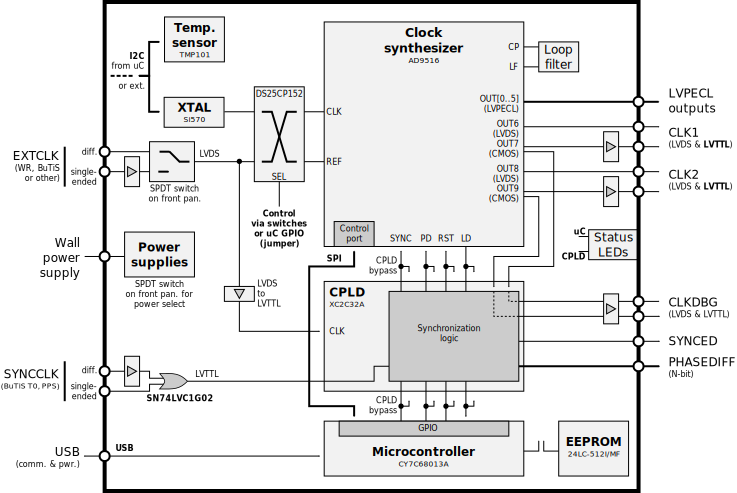
\includegraphics[width=\textwidth]{fig/block-diagram}}
  \caption{\label{fig:block-diagram} Block diagram of the CLOSY3 design}
\end{figure}

\pagebreak
\section{CPLD synchronization logic}
\label{sec:logic}

\subsection{Synchronizing AD9516 outputs}

The AD9516 chip from Analog Devices~\cite{ad9516-3} has a synchronization function
which allows all the outputs of a chip to start clocking synchronously. The AD9516
allows for several ways to synchronize the outputs. These include asserting power down,
reset, or $\overline{SYNC}$ pins, as well as issuing the same commands via
internal bits in the AD9516. For the logic described here, the $\overline{SYNC}$
pin is chosen, as it is the least involved way of performing synchronization while
keeping the settings of the chip.

Upon assertion of the $\overline{SYNC}$ pin, the AD9516's outputs stop clocking for a
predefined amount of time (14 to 15 clocks at the channel divider's inputs + 1 clock at
the channel divider, or VCO divider's inputs, depending on which is used). This delay is
highlighted in Figures 57 and 58 of the AD9516 datasheet~\cite{ad9516-3}.

The principle behind the synchronization logic described here is to assert the
$\overline{SYNC}$ pin, check if an output of an AD9516 chip is synced to
a campus-wide clock (e.g., BuTiS T0, WR PPS) and if it isn't, repeat the process
until the two clocks are in sync. Since all AD9516 outputs are in sync after the
$\overline{SYNC}$ pin is asserted, only one clock is used for synchronization.
When the clock used for synchronization is in sync to the campus-wide clock used for 
synchronization, all clocks output by an AD9516 will be campus-wide synced, since
the AD9516's synchronization function guarantees clocks output by the chip are in sync
after the $\overline{SYNC}$ pin is asserted. See Figures 57 and 58 in the
AD9516 datasheet~\cite{ad9516-3} for more details.

\subsection{Synchronization logic}

The whole concept of the synchronization logic is to allow for an easy-to-change module
that can be used in various places by simply changing VHDL generics at the top-level
of the file prior to compiling the design. This section describes the logic. For
information on how to change the logic, refer to Section~\ref{sec:sources-adapt}.

A block diagram of the synchronization logic described here is shown in
Figure~\ref{fig:logic}. First of all, a clock signal from the AD9516 that has a
frequency which is an integer multiple of the campus-wide clock signal, SYNCCLK, is 
needed for synchronization. A counter clocked on this clock is used to count clocks 
between SYNCCLK rising edges. Either CLK1 or CLK2 from the AD9516 can be used;
which of these is used is done by setting the generic \verb=g_use_clk1= as 
outlined in Section~\ref{sec:sources-adapt}. For simplicity, this document will use 
CLK1 for the rest of the descriptions, but keep in mind that CLK2 can equally be used.
The only thing that is necessary is for this clock to be an integer multiple of SYNCCLK.

If the rising edge of CLK1 is in sync to that of SYNCCLK, seeing as how the frequency of 
CLK1 is an integer multiple of SYNCCLK, a number of CLK1 cycles which is equal to this 
integer multiple should occur between two consecutive SYNCCLK edges. The counter clocked 
on CLK1 is used to check that this number of clock cycles occur. A finite-state machine 
(FSM) clocked on SYNCCLK is used to enable and disable the counter and assert the
$\overline{SYNC}$ pin to the AD9516 to synchronize the outputs when needed. The states of 
the FSM are detailed via Table~\ref{tbl:fsm} and Figure~\ref{fig:fsm}.

The outputs from the block are an active-low SYNC signal to the AD9516 chip and an
epoch signal (SYNCED) that represents a pulse on a selectable epoch period. Note that
the SYNCED output signal is only generated when CLK1 is in sync to SYNCCLK.

\begin{figure}[h]
  \centerline{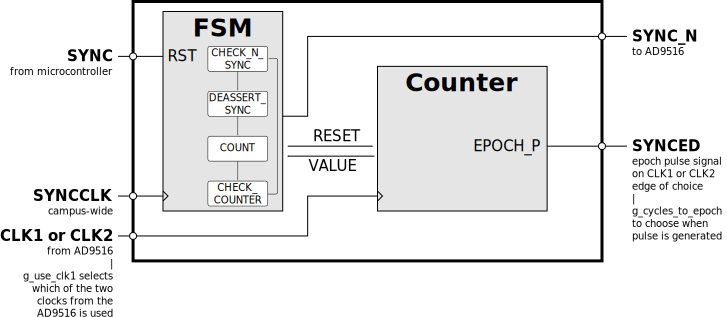
\includegraphics[width=.8\textwidth]{fig/logic}}
  \caption{\label{fig:logic} Block diagram of synchronization logic}
\end{figure}

\begin{table}[h]
  \caption{\label{tbl:fsm} States in the finite-state machine (see also Figure~\ref{fig:fsm})}
  \centerline{
  \rowcolors{2}{white}{gray!25}
  \begin{tabular}{l p{.7\textwidth}}
    \hline
    \multicolumn{1}{c}{\textbf{State}} & \multicolumn{1}{c}{\textbf{Description}} \\
    \hline
    CHECK\_N\_SYNC & Default state. Checks for the internal "synced" signal
                     (asserted in the CHECK\_COUNTER state) and
                     asserts the SYNC\_N signal to the AD9516 if the internal
                     "synced" signal is not asserted. \\
    DEASSERT\_SYNC & De-asserts the SYNC\_N signal to the AD9516. If the signal had
                     previously been asserted within CHECK\_N\_SYNC, the AD9516 outputs
                     will start clocking after the delay specified in the
                     datasheet~\cite{ad9516-3}. This will prepare for the counter
                     starting to count up on the next state. \\
    COUNT          & De-assert the counter reset signal, which allows the counter to
                     start counting up. At the end of this state, if CLK1 or CLK2 
                     (whichever is used) is in sync to SYNCCLK, the counter should have
                     returned to zero. \\
   CHECK\_COUNTER  & Check whether the counter is zero and assert the internal "synced"
                     signal, which is used in the starting state of the FSM to see if
                     the SYNC\_N signal to the AD9516 should be asserted. \\
    \hline
  \end{tabular}
  }
\end{table}

Note that when the \textbf{active-low} SYNC signal from the microcontroller is asserted,
the FSM resets into its default state (CHECK\_N\_SYNC).

\begin{figure}[h]
  \centerline{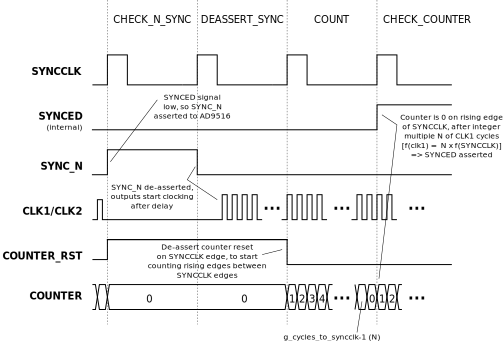
\includegraphics[width=\textwidth]{fig/fsm}}
  \caption{\label{fig:fsm} Functioning of the synchronization logic}
\end{figure}

\section{Testing}
\label{sec:testing}

The synchronization logic was tested using two CLOSY2 boards and the CPLDs placed on them
connected with wires to two AD9516-3 development boards. A single function generator
provided both a 10~KHz SYNCCLK signal for the synchronization logic and a 10~MHz reference 
for the AD9516-3 development boards. The function generator's outputs were connected
with splitters and cables to the two CLOSY2s and the development boards respectively.

The test yielded that the functionality of the logic is either incorrect, or that there
is another problem related to the wiring between the equipment used during testing. The
hunch about a wiring-related problem is due to the fact that the synchronization logic 
consistently asserted the $\overline{SYNC}$ pin to the AD9516 development boards during
testing, but this consistent assertion of the pin was done in a random manner.

More testing should be performed, possible checking the state of the counter on SYNCCLK
edges.

\textbf{Another idea for implementation, which would require a larger CPLD with more
macrocells, is to modify the FSM to de-assert the $\overline{SYNC}$ pin to the AD9516
14 clock cycles before the SYNCCLK edge.} This is however only an idea to be tested.

\section{VHDL source files}
\label{sec:sources}

\subsection{Where to get the source files}
\label{sec:sources-where}

The source files for the synchronization logic can be found on the GSI server at
the following path:

\begin{center}
\begin{verbatim}
K:\GsiJob\CLOSY\CLOSY3\closy3-gw
\end{verbatim}
\end{center}

The folder structure for the files can be found in Table~\ref{tbl:folder-struct}.

\begin{table}[h]
  \caption{\label{tbl:folder-struct} Folder structure for the source files}
  \centerline {
  \rowcolors{2}{white}{gray!25}
  \begin{tabular}{l p{.7\textwidth}}
    \hline
    \multicolumn{1}{c}{\textbf{Folder}} & \multicolumn{1}{c}{\textbf{Description}} \\
    \hline
    doc/ & Documentation files for the logic (LaTeX source files for this document) \\
    sim/ & Simulation testbench (closy3\_cbm/ sub-folder) \\
    syn/ & ISE project file and synthesis-specific files (closy3\_cbm/ sub-folder \\
    top/ & Top-level VHDL file and UCF constraints file \\
    \hline
  \end{tabular}
  }
\end{table}

\subsection{How to adapt the logic}
\label{sec:sources-adapt}

In order to adapt the CLOSY3 synchronization logic for new uses, the generics of the
entity can be changed to allow for new CLK1 and CLK2 frequencies. The listing below shows 
where the generics can be found in the VHDL file and Table~\ref{tbl:generics} lists the 
generics and their settings.

\begin{small}
\begin{center}
\begin{verbatim}
entity closy3_cbm is
  generic
  (
    -- Use clk1_i for synchronization mechanism; else, use clk2_i
    g_use_clk1 : boolean := true;
    
    -- clk_for_sync cycles between syncclk_i rising edges
    g_cycles_to_syncclk : natural := 6250;
    
    -- clk_for_sync cycles to epoch
    g_cycles_to_epoch   : natural := 4096
  );
  port
  (
\end{verbatim}
\end{center}
\end{small}

The default values shown above pertain to a SYNCCLK frequency of 10~KHz (the BuTiS T0 
clock), using a 62.5~MHz CLK1 as the synchronization clock (\verb-g_use_clk1 = true-).
Since 62.5~MHz divided by 6250 yields 10~KHz, the counter should wrap around every
6250 cycles to be in sync. The epoch pulse is generated every 4096 cycles of the 62.5~MHz
CLK1 signal, i.e., every 65.536~$\mu$s.

\begin{table}[h]
  \caption{\label{tbl:generics} Generics at the top-level of the VHDL file}
  \centerline{
  \rowcolors{2}{white}{gray!25}
  \begin{tabular}{l p{.7\textwidth}}
    \hline
    \multicolumn{1}{c}{\textbf{Generic}} & \multicolumn{1}{c}{\textbf{Description}} \\
    \hline
    g\_use\_clk1 & Selects whether to use CLK1 or CLK2 from the AD9516 \newline
                   \textbf{true} -- use CLK1 \newline
                   \textbf{false} -- use CLK2 \\
    g\_cycles\_to\_syncclk & Number of cycles of CLK1 or CLK2 (based on previous generic)
                            between SYNCCLK cycles. This basically selects the modulus
                            of the counter (where it should wrap around to zero). \\
    g\_cycles\_to\_epoch & Number of cycles until epoch generation. A
                           single-clock-cycle pulse will be generated on the SYNCED
                           output of the CPLD to signal the epoch once every
                           \textit{g\_cycles\_to\_epoch} cycles. 
                           Note that the epoch pulse is generated only if the clocks
                           are in sync. \\
    \hline
  \end{tabular}
  }
\end{table}

\subsection{Stub files}
\label{sec:sources-stubs}

A couple of stub files are provided in the \verb=top/= folder of the folder structure.
These files provide a starting point for new gateware developments for the CLOSY3.
The \verb=closy3_stub.vhd= file declares the entity and the pins as they appear in the 
schematics at the date of writing of this document. Correspondingly, the 
\verb=closy3_stub.ucf= file declares the pinout of the CPLD as it appears in the 
schematics at the date of writing of this document.

\textbf{New developments should be done by copying the stub files and modifying the 
copies.}

%==============================================================================
% Bibliography
%==============================================================================
\pagebreak
\bibliographystyle{ieeetr}
\bibliography{closy3-cbm}
\addcontentsline{toc}{section}{References}

\end{document}
